\documentclass{article}

\usepackage[top=2.54cm, left=2.54cm, right=2.54cm, bottom=2.54cm]{geometry}
\usepackage{amsmath}
\usepackage{booktabs}
\usepackage{hyperref}
\usepackage{multicol}
\hypersetup{colorlinks=true, urlcolor=blue,}
\usepackage[svgnames]{xcolor}
\usepackage{graphicx}

\begin{document}
\hrule
\begin{center}
\large {Quantum Harmonic Oscillator}\\ \large{and Hermite Polynomials}
\end{center}

\hrule
\vspace{1pt}
\hrule height 1pt

\section{Introduction}
The Schrodinger equation for a harmonic oscillator may be obtained by using the classical spring potential
given by

\begin{equation}
\label{eq:1}
V(X) = \frac{1}{2}mw^2x^2
\end{equation}
where m is the mass, $x$ is the position, and $w$ is the angular frequency given by

\begin{equation}
\label{eq:2}
w = \sqrt{\frac{k}{m}}
\end{equation}

\noindent
The Schrodinger equation with this form of potential is described by
\begin{equation}
\label{eq:3}
-\frac{\hbar^2}{2m} 
\frac{d^2\\Psi(x)}{dx^2} + V(x)\Psi(x) = E\Psi(x)
\end{equation}
where $V(x)$ is given by Eq. \eqref{eq:1} Since the derivative of the wavefunction must give back the square of $x$ plus
a constant times the original function, then the form

\begin{equation}
\label{eq:4}
\Psi(x) = C e^{-\alpha x^2 / 2}
\end{equation}
is suggested.\\

\noindent
Note that this form which is in a Gaussian form satisfies the requirement of going to zero at infinity, making
it possible to normalize the wavefunction. Substituting this function into the Schrodinger equation and
fitting the boundary conditions leads to the ground state energy for the quantum harmonic oscillator given
by
\begin{equation}
\label{eq:5}
E_{0} = \frac{\hbar w}{2}
\end{equation}
The general solution to the Schrodinger equation leads to a sequence of evenly spaced energy levels characterized
by a quantum number n as shown in Fig. \ref{fig:1}.\\

\begin{figure}[h]
\begin{center}
\includegraphics[scale=0.65]{./potwell}
\end{center}
\caption{Image Credit: \url{www.hyperphysics.com}}
\label{fig:1}
\end{figure}

\noindent
The wavefunctions for the quantum harmonic oscillator contain the Gaussian form which allows them to
satisfy the necessary boundary conditions at infinity. In the wavefunction associated with a given value of the
quantum number n, the Gaussian is multiplied by a polynomial of order n called a \textbf{Hermite polynomial}.
The expressions are simplified by making the substitution

\begin{equation}
\label{eq:6}
y = \sqrt{\alpha}x
\end{equation}

where $\alpha= \frac{mw}{\hbar}$. The general formula for the normalized wavefunction is then

\begin{equation}
\label{eq:7}
\Psi(x) = (y) = (\frac{\alpha}{\pi})^{1/4} \frac{1}{\sqrt{2^n !}} H_{n}(y) e^{-y^2 / 2}
\end{equation}
where $H_{n}(y)$ are the Hermite Polynomials.


\section{Solutions to the Schrodinger Equation}
The Schrodinger equation for a harmonic oscillator may be solved to give the wavefunctions illustrated in Fig. \ref{fig:2}.

\begin{figure}[h]
\begin{center}
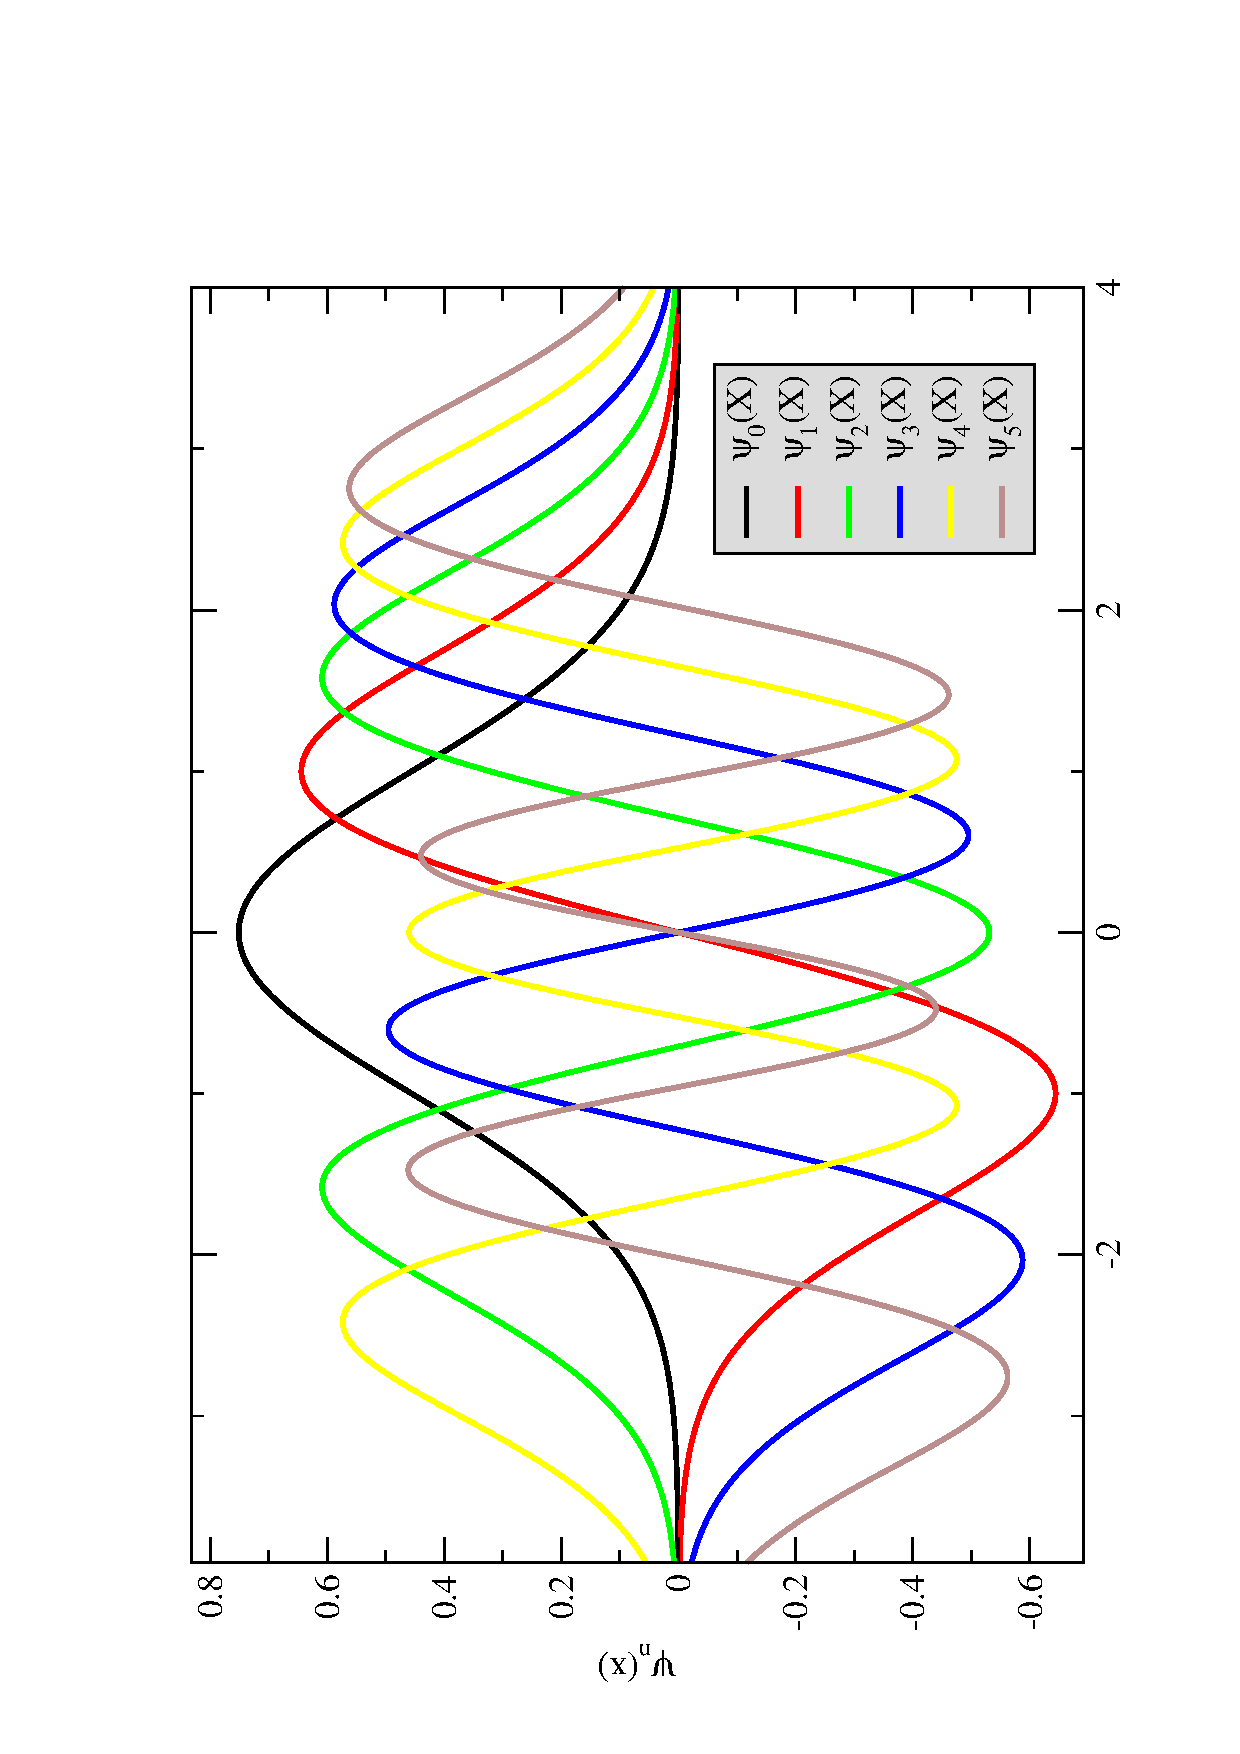
\includegraphics[scale=0.4, angle=-90]{./hermite}
\end{center}
\label{fig:2}
\end{figure}

\noindent
Figure 2: Solutions to the Schrodinger Equation for the first six energy states gives the normalized wavefunctions
shown here.\\

\noindent
The probability of finding the oscillator at any given value of $x$ is the square of the wavefunction. Note that
the wavefunctions for higher $n$ have more “humps” within the potential well. This corresponds to a shorter
wavelength and therefore by the deBroglie relationship they may be seen to have a higher momentum and
therefore higher energy.\\

\noindent
The most probable value of position for the lower states is very different from the classical harmonic oscillator
where it spends more time near the end of its motion. But as the quantum number increases, the probability
distribution becomes more like that of the classical oscillator.\pagebreak

\noindent
When the Schrodinger equation for the harmonic oscillator is solved by a series method, the solutions contain
this set of polynomials, named the Hermite polynomials. The values for n for the first six are shown in Table \ref{table:1}.\\


\begin{table}[h]
\centering
\begin{tabular}{ l l l } 
\multicolumn{3}{c}{Table 1: blah}\\
\hline \hline
$n$ & $H_n(y)$ & $E_n$\\
 \hline
 0 & 1 										& $\frac{1}{2}\hbar w$\\\noalign{\smallskip}
 1 & $2y$ 									& $\frac{3}{2}\hbar w$\\\noalign{\smallskip}
 2 & $4y^2 - 2$ 						& $\frac{5}{2}\hbar w$\\\noalign{\smallskip}
 3 & $8y^3 - 12y$ 						& $\frac{7}{2}\hbar w$\\\noalign{\smallskip}
 4 & $16y^4 - 48y^2 + 12y$ 		& $\frac{9}{2}\hbar w$\\\noalign{\smallskip}
 5 & $32y^5 - 160y^3 + 120y$ 	& $\frac{11}{2}\hbar w$\\\noalign{\smallskip}
 \hline
\end{tabular}
\label{table:1}
\end{table}


\noindent
The wavefunctions for the quantum harmonic oscillator contain the Gaussian form which allows them to
satisfy the necessary boundary conditions at infinity. In the wavefunction associated with a given value of
the quantum number $n$, the Gaussian is multiplied by a polynomial of order $n$ (the Hermite polynomials
above) and the constants necessary to normalize the wavefunctions.

\end{document}
